\subsection{Limitationer ved trådløs energioverførelse }
Trådløs energioverførsel indeholder mange muligheder, og der er stor plads til videreudvikling. Med projektets fokus på trådløs opladning af mobiltelefoner, vil der i dette afsnit blive sat fokus på begrænsninger og ulemper ved induktiv energioverførsel. Fokusset indenfor begrænsningerne vil ligge ved selve energioverførslen angående distance og effekt. Derudover vil betydningen af frekvens, tab af energi i form af varme, samt standarder for WPT blive beskrevet.

Effekten for opladningen afhænger af en række forskellige faktorer bl.a. distancen mellem transmitter og modtager, størrelsen af frekvensen og hvor stærk en strøm, der skal overføres. I dag er teknologien for IPT (Inductive Power Transfer) i stand til at holde en effektivitet på 90 procent ved en distance på op til 10cm. Dette betyder, at der sker et energitab på omkring 10 procent, som omdannes til varmeenergi, ellers optages af forstyrrende elementer. Størrelsen af spolerne og frekvensen influerer også til størrelsen af den magnetiske flux, som dannes ved spolerne.

Da der sker et energitab på omkring 10 procent for IPT ved en distance på 10cm, så kunne det undersøges, hvorvidt tabet forandre sig ved yderligere distance, eller om det forbliver ved de 10 procent.

Ved de følgende tre figurer ses der bort fra de kryds-formede punkter.

\begin{figure}[H]
\centering
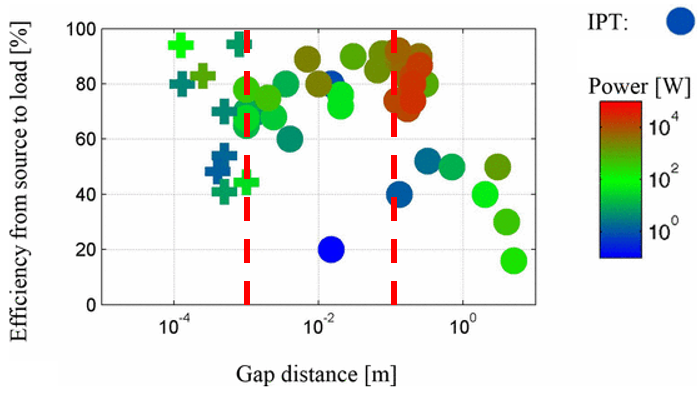
\includegraphics[scale=0.5]{Vildledning/Schematics/Effektivitet_vs_gap.png}
\caption{Figur Effektivitet}
\end{figure}

Figur X viser, hvordan effektiviteten ændre sig ved forskellige distancer. Ved grafen dannes der to grupper af punkter; ét omkring 1mm og ét omkring 10cm. Punkterne er inddelt i forskellige farver, som indikerer effekten for det enkelte punkt. De lave effekter på omkring 1W har en effektivitet på 20 procent ved en distance på 1cm, hvorefter det siger i effektivitet, når distancen øges, men forbliver under 60 procent. For effekter på omkring 100W er det mest centreret ved 1mm med en effektivitet mellem 65 til 80 procent. Andre punkter med denne effekt befinder sig med en distance på 1 til 10m mellem transmitter og modtager. Ved 1m er effektiviteten på 50 procent, men falder hurtigt og er på under 15 procent inden de 10m er nået. Ved en effekt på 10kW er punkterne centreret ved en distance på 10cm, hvor effektiviteten varrierer fra 65 procent og op til 90 procent.

Arealet for transmitteren og modtageren har også betydning for, hvor meget energioverførsel der finder sted. Derudover er det heller ikke ligegyldigt, hvor stor en effekt der bliver udsendt. Figur X viser, hvordan sammenhængen mellem spolernes areal og den udsendte effekt spiller en rolle for effektiviteten.

\begin{figure}[H]
\centering
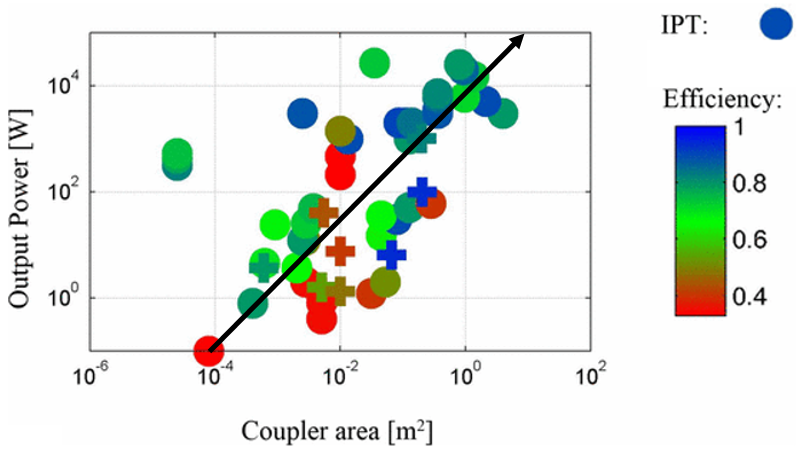
\includegraphics[scale=0.5]{Vildledning/Schematics/Power_vs_coupler-area.png}
\caption{Figur Power}
\end{figure}

Punkterne følger groft en linier funktion, hvor effekten stiger i takt med, at spolernes areal forstørres. Punkternes farver angiver effektiviteten for energioverførslen, hvor rød er $\leq 40$ procent, mens blå er $\geq 80$ procent. Effektiviteten befinder sig i det røde felt, når spolernes areal er små, samt effekten er lav. Modsat er effektiviteten oppe i det blå område, når spolernes areal er store, og der bliver udsendt en høj effekt. Angående areal, så er det ikke kun størrelsen på spolerne der tæller, men også hvordan modtageren er placeret i forhold til transmitteren. Hvis de to spoler er parallelle, vil de have den mest optimale stilling, men hvis modtageren står vinklet på transmitteren, vil nogle af de magnetiske feltlinjer forbigå modtageren, og effektiviteten vil derved blive mindsket.

For at undgå for meget energitab, så skal der benyttes en optimal frekvens for den energi, der skal overføres trådløst.

\begin{figure}[H]
\centering
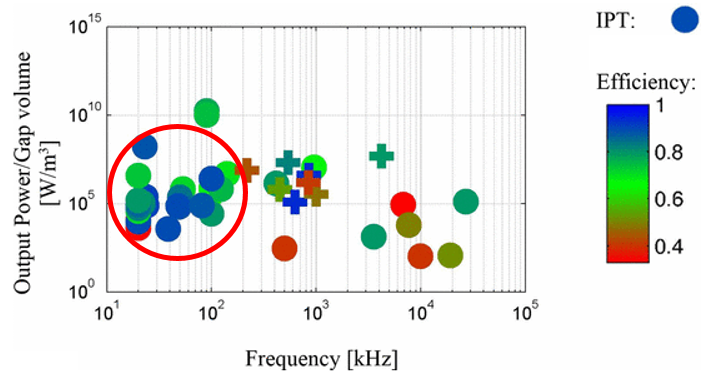
\includegraphics[scale=0.5]{Vildledning/Schematics/Power_vs_frekvens.png}
\caption{Figur Frekvens}
\end{figure}

Figur X viser, hvordan effektiviteten for trådløs energioverførsel udfolder sig ved forskellige frekvenser og forholdet mellem den udsendte effekt og magnetfeltets vej. Magnetfeltets vej er angivet som spolernes areal ganget med distancen for energioverførslen. Punkterne på figuren centrerer sig omkring to punkter; ét ved en frekvens mellem 20 og 100kHz og et ved en frekvens på 4 til 10MHz. Effektiviteten for de to områder er dog stor, hvor de høje frekvenser ligger på 50 procent eller under, mens de mindre frekvenser ligger på 60 procent og op til 90 procent.

Siden 2005 og til nu har IPT teknologien udviklet sig, så den gennemsnitlige frekvens og energiudnyttelse forøget ca. ti foldigt. Denne from for udvikling kan også hos transiter, dette fænomen hedder Moore's lov. Denne udvikling regnes der også at forekomme de næste år indenfor WPT. 

\begin{figure}[H]
\centering
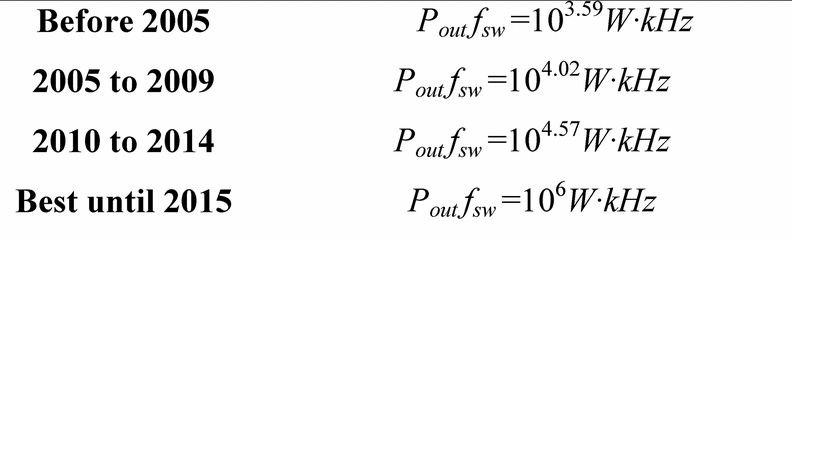
\includegraphics[scale=0.5]{Vildledning/Schematics/frekvens_energi}
\caption{Frekvens/energi Udvikling}
\end{figure}
Med øgende frekvens og energi udbytte, med kommer der flere samfundsmæssige begrænsninger. Disse begrænsninger styres af nogle standarter kaldt Qi. 

\subsection{Qi}
For at få implementeret trådløs opladning, så skal produkterne overholde bestemte systemkrav, for at opladningen skal kunne fungere optimalt eller overhovedet fungere.

Wireless power consortium er en samlet organisation af forskellige virksomheder, som arbejder med trådløs opladning indenfor mange forskellige produkter. De har igennem denne organisation opsat det, de kalder Qi-standarderne, som beskriver hvilke systemkrav der skal opfyldes, og hvilke dele der skal implementeres i produkterne, før de er kompatible til trådløs opladning.

For at en trådløs opladning kan finde sted, skal der være en transmitter, der udsender strømmen, mens der i modsatte ende skal være en modtager, der opfanger strømmen og oplader produktet. For at produktets opladning skal godkendes af Qi-standarderne, skal transmitteren indeholde en brugerflade, som kan koples sammen med alle godkendte modtagere. Derudover skal modtageren kunne sende oplysningerne omkring opladningen tilbage til transmitteren, så den modtager data, den kan bearbejde.
